% Created by tikzDevice version 0.12 on 2019-08-24 14:26:37
% !TEX encoding = UTF-8 Unicode
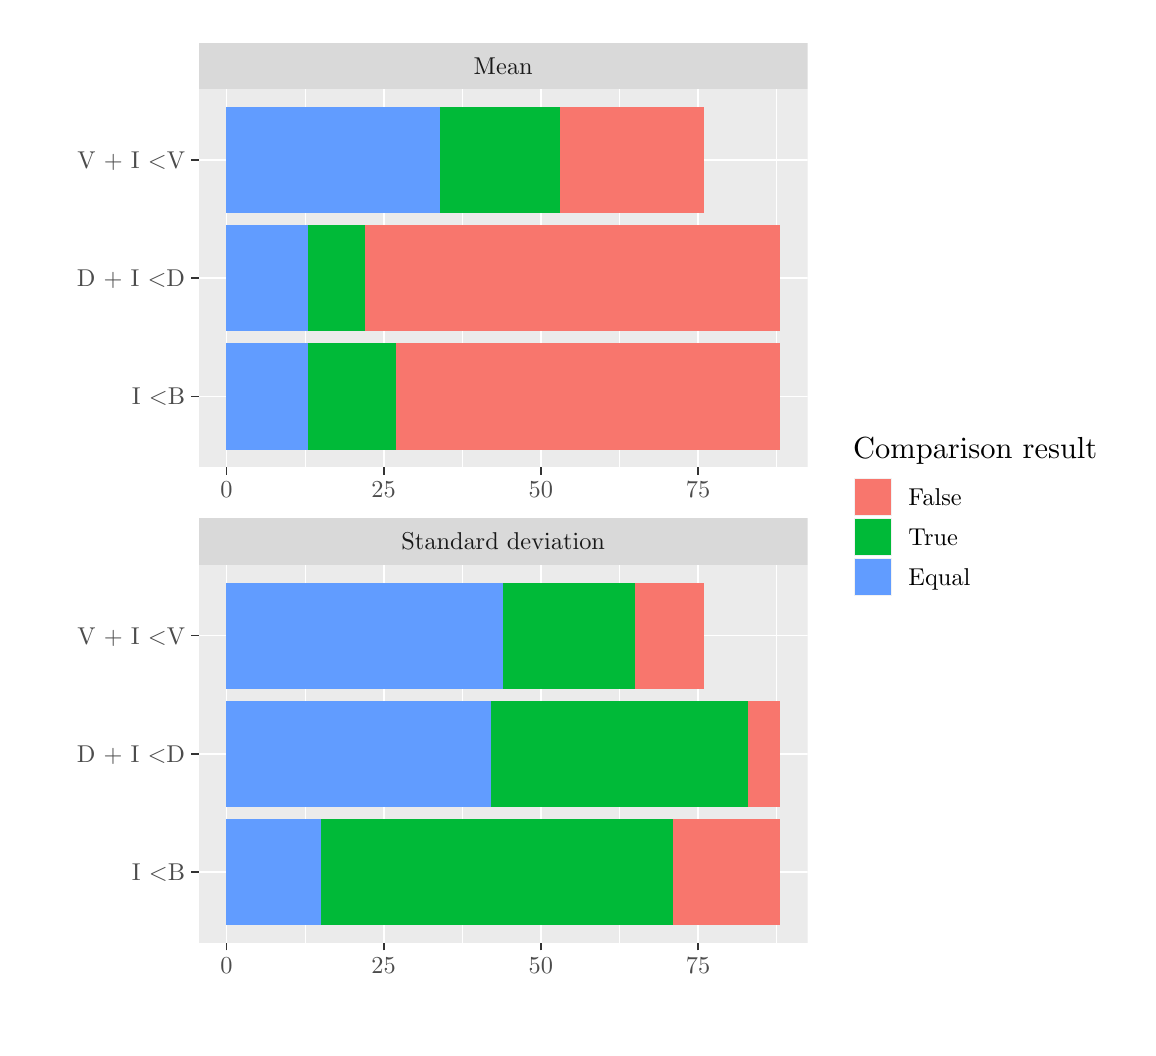
\begin{tikzpicture}[x=1pt,y=1pt]
\definecolor{fillColor}{RGB}{255,255,255}
\path[use as bounding box,fill=fillColor,fill opacity=0.00] (0,0) rectangle (397.48,361.35);
\begin{scope}
\path[clip] (  0.00,  0.00) rectangle (397.48,361.35);
\definecolor{drawColor}{RGB}{255,255,255}
\definecolor{fillColor}{RGB}{255,255,255}

\path[draw=drawColor,line width= 0.6pt,line join=round,line cap=round,fill=fillColor] (  0.00,  0.00) rectangle (397.48,361.35);
\end{scope}
\begin{scope}
\path[clip] ( 61.82,202.51) rectangle (281.82,339.05);
\definecolor{fillColor}{gray}{0.92}

\path[fill=fillColor] ( 61.82,202.51) rectangle (281.82,339.05);
\definecolor{drawColor}{RGB}{255,255,255}

\path[draw=drawColor,line width= 0.3pt,line join=round] (100.23,202.51) --
	(100.23,339.05);

\path[draw=drawColor,line width= 0.3pt,line join=round] (157.05,202.51) --
	(157.05,339.05);

\path[draw=drawColor,line width= 0.3pt,line join=round] (213.87,202.51) --
	(213.87,339.05);

\path[draw=drawColor,line width= 0.3pt,line join=round] (270.69,202.51) --
	(270.69,339.05);

\path[draw=drawColor,line width= 0.6pt,line join=round] ( 61.82,228.11) --
	(281.82,228.11);

\path[draw=drawColor,line width= 0.6pt,line join=round] ( 61.82,270.78) --
	(281.82,270.78);

\path[draw=drawColor,line width= 0.6pt,line join=round] ( 61.82,313.45) --
	(281.82,313.45);

\path[draw=drawColor,line width= 0.6pt,line join=round] ( 71.82,202.51) --
	( 71.82,339.05);

\path[draw=drawColor,line width= 0.6pt,line join=round] (128.64,202.51) --
	(128.64,339.05);

\path[draw=drawColor,line width= 0.6pt,line join=round] (185.46,202.51) --
	(185.46,339.05);

\path[draw=drawColor,line width= 0.6pt,line join=round] (242.28,202.51) --
	(242.28,339.05);
\definecolor{fillColor}{RGB}{97,156,255}

\path[fill=fillColor] ( 71.82,208.91) rectangle (101.37,247.31);
\definecolor{fillColor}{RGB}{0,186,56}

\path[fill=fillColor] (101.37,208.91) rectangle (133.19,247.31);
\definecolor{fillColor}{RGB}{248,118,109}

\path[fill=fillColor] (133.19,208.91) rectangle (271.82,247.31);
\definecolor{fillColor}{RGB}{97,156,255}

\path[fill=fillColor] ( 71.82,251.58) rectangle (101.37,289.98);
\definecolor{fillColor}{RGB}{0,186,56}

\path[fill=fillColor] (101.37,251.58) rectangle (121.82,289.98);
\definecolor{fillColor}{RGB}{248,118,109}

\path[fill=fillColor] (121.82,251.58) rectangle (271.82,289.98);
\definecolor{fillColor}{RGB}{97,156,255}

\path[fill=fillColor] ( 71.82,294.25) rectangle (149.09,332.65);
\definecolor{fillColor}{RGB}{0,186,56}

\path[fill=fillColor] (149.09,294.25) rectangle (192.28,332.65);
\definecolor{fillColor}{RGB}{248,118,109}

\path[fill=fillColor] (192.28,294.25) rectangle (244.55,332.65);
\end{scope}
\begin{scope}
\path[clip] ( 61.82, 30.72) rectangle (281.82,167.26);
\definecolor{fillColor}{gray}{0.92}

\path[fill=fillColor] ( 61.82, 30.72) rectangle (281.82,167.26);
\definecolor{drawColor}{RGB}{255,255,255}

\path[draw=drawColor,line width= 0.3pt,line join=round] (100.23, 30.72) --
	(100.23,167.26);

\path[draw=drawColor,line width= 0.3pt,line join=round] (157.05, 30.72) --
	(157.05,167.26);

\path[draw=drawColor,line width= 0.3pt,line join=round] (213.87, 30.72) --
	(213.87,167.26);

\path[draw=drawColor,line width= 0.3pt,line join=round] (270.69, 30.72) --
	(270.69,167.26);

\path[draw=drawColor,line width= 0.6pt,line join=round] ( 61.82, 56.32) --
	(281.82, 56.32);

\path[draw=drawColor,line width= 0.6pt,line join=round] ( 61.82, 98.99) --
	(281.82, 98.99);

\path[draw=drawColor,line width= 0.6pt,line join=round] ( 61.82,141.66) --
	(281.82,141.66);

\path[draw=drawColor,line width= 0.6pt,line join=round] ( 71.82, 30.72) --
	( 71.82,167.26);

\path[draw=drawColor,line width= 0.6pt,line join=round] (128.64, 30.72) --
	(128.64,167.26);

\path[draw=drawColor,line width= 0.6pt,line join=round] (185.46, 30.72) --
	(185.46,167.26);

\path[draw=drawColor,line width= 0.6pt,line join=round] (242.28, 30.72) --
	(242.28,167.26);
\definecolor{fillColor}{RGB}{97,156,255}

\path[fill=fillColor] ( 71.82, 37.12) rectangle (105.91, 75.52);
\definecolor{fillColor}{RGB}{0,186,56}

\path[fill=fillColor] (105.91, 37.12) rectangle (233.19, 75.52);
\definecolor{fillColor}{RGB}{248,118,109}

\path[fill=fillColor] (233.19, 37.12) rectangle (271.82, 75.52);
\definecolor{fillColor}{RGB}{97,156,255}

\path[fill=fillColor] ( 71.82, 79.79) rectangle (167.28,118.19);
\definecolor{fillColor}{RGB}{0,186,56}

\path[fill=fillColor] (167.28, 79.79) rectangle (260.46,118.19);
\definecolor{fillColor}{RGB}{248,118,109}

\path[fill=fillColor] (260.46, 79.79) rectangle (271.82,118.19);
\definecolor{fillColor}{RGB}{97,156,255}

\path[fill=fillColor] ( 71.82,122.46) rectangle (171.82,160.86);
\definecolor{fillColor}{RGB}{0,186,56}

\path[fill=fillColor] (171.82,122.46) rectangle (219.55,160.86);
\definecolor{fillColor}{RGB}{248,118,109}

\path[fill=fillColor] (219.55,122.46) rectangle (244.55,160.86);
\end{scope}
\begin{scope}
\path[clip] ( 61.82,167.26) rectangle (281.82,184.06);
\definecolor{fillColor}{gray}{0.85}

\path[fill=fillColor] ( 61.82,167.26) rectangle (281.82,184.06);
\definecolor{drawColor}{gray}{0.10}

\node[text=drawColor,anchor=base,inner sep=0pt, outer sep=0pt, scale=  0.88] at (171.82,172.63) {Standard deviation};
\end{scope}
\begin{scope}
\path[clip] ( 61.82,339.05) rectangle (281.82,355.85);
\definecolor{fillColor}{gray}{0.85}

\path[fill=fillColor] ( 61.82,339.05) rectangle (281.82,355.85);
\definecolor{drawColor}{gray}{0.10}

\node[text=drawColor,anchor=base,inner sep=0pt, outer sep=0pt, scale=  0.88] at (171.82,344.42) {Mean};
\end{scope}
\begin{scope}
\path[clip] (  0.00,  0.00) rectangle (397.48,361.35);
\definecolor{drawColor}{gray}{0.20}

\path[draw=drawColor,line width= 0.6pt,line join=round] ( 71.82, 27.97) --
	( 71.82, 30.72);

\path[draw=drawColor,line width= 0.6pt,line join=round] (128.64, 27.97) --
	(128.64, 30.72);

\path[draw=drawColor,line width= 0.6pt,line join=round] (185.46, 27.97) --
	(185.46, 30.72);

\path[draw=drawColor,line width= 0.6pt,line join=round] (242.28, 27.97) --
	(242.28, 30.72);
\end{scope}
\begin{scope}
\path[clip] (  0.00,  0.00) rectangle (397.48,361.35);
\definecolor{drawColor}{gray}{0.30}

\node[text=drawColor,anchor=base,inner sep=0pt, outer sep=0pt, scale=  0.88] at ( 71.82, 19.71) {0};

\node[text=drawColor,anchor=base,inner sep=0pt, outer sep=0pt, scale=  0.88] at (128.64, 19.71) {25};

\node[text=drawColor,anchor=base,inner sep=0pt, outer sep=0pt, scale=  0.88] at (185.46, 19.71) {50};

\node[text=drawColor,anchor=base,inner sep=0pt, outer sep=0pt, scale=  0.88] at (242.28, 19.71) {75};
\end{scope}
\begin{scope}
\path[clip] (  0.00,  0.00) rectangle (397.48,361.35);
\definecolor{drawColor}{gray}{0.20}

\path[draw=drawColor,line width= 0.6pt,line join=round] ( 71.82,199.76) --
	( 71.82,202.51);

\path[draw=drawColor,line width= 0.6pt,line join=round] (128.64,199.76) --
	(128.64,202.51);

\path[draw=drawColor,line width= 0.6pt,line join=round] (185.46,199.76) --
	(185.46,202.51);

\path[draw=drawColor,line width= 0.6pt,line join=round] (242.28,199.76) --
	(242.28,202.51);
\end{scope}
\begin{scope}
\path[clip] (  0.00,  0.00) rectangle (397.48,361.35);
\definecolor{drawColor}{gray}{0.30}

\node[text=drawColor,anchor=base,inner sep=0pt, outer sep=0pt, scale=  0.88] at ( 71.82,191.50) {0};

\node[text=drawColor,anchor=base,inner sep=0pt, outer sep=0pt, scale=  0.88] at (128.64,191.50) {25};

\node[text=drawColor,anchor=base,inner sep=0pt, outer sep=0pt, scale=  0.88] at (185.46,191.50) {50};

\node[text=drawColor,anchor=base,inner sep=0pt, outer sep=0pt, scale=  0.88] at (242.28,191.50) {75};
\end{scope}
\begin{scope}
\path[clip] (  0.00,  0.00) rectangle (397.48,361.35);
\definecolor{drawColor}{gray}{0.30}

\node[text=drawColor,anchor=base east,inner sep=0pt, outer sep=0pt, scale=  0.88] at ( 56.87,225.08) {I \textless B};

\node[text=drawColor,anchor=base east,inner sep=0pt, outer sep=0pt, scale=  0.88] at ( 56.87,267.75) {D + I \textless D};

\node[text=drawColor,anchor=base east,inner sep=0pt, outer sep=0pt, scale=  0.88] at ( 56.87,310.42) {V + I \textless V};
\end{scope}
\begin{scope}
\path[clip] (  0.00,  0.00) rectangle (397.48,361.35);
\definecolor{drawColor}{gray}{0.20}

\path[draw=drawColor,line width= 0.6pt,line join=round] ( 59.07,228.11) --
	( 61.82,228.11);

\path[draw=drawColor,line width= 0.6pt,line join=round] ( 59.07,270.78) --
	( 61.82,270.78);

\path[draw=drawColor,line width= 0.6pt,line join=round] ( 59.07,313.45) --
	( 61.82,313.45);
\end{scope}
\begin{scope}
\path[clip] (  0.00,  0.00) rectangle (397.48,361.35);
\definecolor{drawColor}{gray}{0.30}

\node[text=drawColor,anchor=base east,inner sep=0pt, outer sep=0pt, scale=  0.88] at ( 56.87, 53.29) {I \textless B};

\node[text=drawColor,anchor=base east,inner sep=0pt, outer sep=0pt, scale=  0.88] at ( 56.87, 95.96) {D + I \textless D};

\node[text=drawColor,anchor=base east,inner sep=0pt, outer sep=0pt, scale=  0.88] at ( 56.87,138.63) {V + I \textless V};
\end{scope}
\begin{scope}
\path[clip] (  0.00,  0.00) rectangle (397.48,361.35);
\definecolor{drawColor}{gray}{0.20}

\path[draw=drawColor,line width= 0.6pt,line join=round] ( 59.07, 56.32) --
	( 61.82, 56.32);

\path[draw=drawColor,line width= 0.6pt,line join=round] ( 59.07, 98.99) --
	( 61.82, 98.99);

\path[draw=drawColor,line width= 0.6pt,line join=round] ( 59.07,141.66) --
	( 61.82,141.66);
\end{scope}
\begin{scope}
\path[clip] (  0.00,  0.00) rectangle (397.48,361.35);
\definecolor{fillColor}{RGB}{255,255,255}

\path[fill=fillColor] (292.82,150.19) rectangle (391.98,219.58);
\end{scope}
\begin{scope}
\path[clip] (  0.00,  0.00) rectangle (397.48,361.35);
\definecolor{drawColor}{RGB}{0,0,0}

\node[text=drawColor,anchor=base west,inner sep=0pt, outer sep=0pt, scale=  1.10] at (298.32,205.53) {Comparison result};
\end{scope}
\begin{scope}
\path[clip] (  0.00,  0.00) rectangle (397.48,361.35);
\definecolor{drawColor}{RGB}{255,255,255}
\definecolor{fillColor}{gray}{0.95}

\path[draw=drawColor,line width= 0.6pt,line join=round,line cap=round,fill=fillColor] (298.32,184.60) rectangle (312.78,199.06);
\end{scope}
\begin{scope}
\path[clip] (  0.00,  0.00) rectangle (397.48,361.35);
\definecolor{fillColor}{RGB}{248,118,109}

\path[fill=fillColor] (299.03,185.31) rectangle (312.07,198.34);
\end{scope}
\begin{scope}
\path[clip] (  0.00,  0.00) rectangle (397.48,361.35);
\definecolor{drawColor}{RGB}{255,255,255}
\definecolor{fillColor}{gray}{0.95}

\path[draw=drawColor,line width= 0.6pt,line join=round,line cap=round,fill=fillColor] (298.32,170.15) rectangle (312.78,184.60);
\end{scope}
\begin{scope}
\path[clip] (  0.00,  0.00) rectangle (397.48,361.35);
\definecolor{fillColor}{RGB}{0,186,56}

\path[fill=fillColor] (299.03,170.86) rectangle (312.07,183.89);
\end{scope}
\begin{scope}
\path[clip] (  0.00,  0.00) rectangle (397.48,361.35);
\definecolor{drawColor}{RGB}{255,255,255}
\definecolor{fillColor}{gray}{0.95}

\path[draw=drawColor,line width= 0.6pt,line join=round,line cap=round,fill=fillColor] (298.32,155.69) rectangle (312.78,170.15);
\end{scope}
\begin{scope}
\path[clip] (  0.00,  0.00) rectangle (397.48,361.35);
\definecolor{fillColor}{RGB}{97,156,255}

\path[fill=fillColor] (299.03,156.41) rectangle (312.07,169.44);
\end{scope}
\begin{scope}
\path[clip] (  0.00,  0.00) rectangle (397.48,361.35);
\definecolor{drawColor}{RGB}{0,0,0}

\node[text=drawColor,anchor=base west,inner sep=0pt, outer sep=0pt, scale=  0.88] at (318.28,188.80) {False};
\end{scope}
\begin{scope}
\path[clip] (  0.00,  0.00) rectangle (397.48,361.35);
\definecolor{drawColor}{RGB}{0,0,0}

\node[text=drawColor,anchor=base west,inner sep=0pt, outer sep=0pt, scale=  0.88] at (318.28,174.34) {True};
\end{scope}
\begin{scope}
\path[clip] (  0.00,  0.00) rectangle (397.48,361.35);
\definecolor{drawColor}{RGB}{0,0,0}

\node[text=drawColor,anchor=base west,inner sep=0pt, outer sep=0pt, scale=  0.88] at (318.28,159.89) {Equal};
\end{scope}
\end{tikzpicture}
